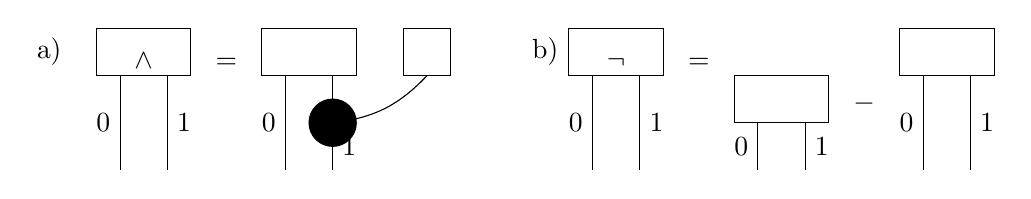
\begin{tikzpicture}[scale=0.3] 

\node at (-12,2) [above]  {a)};

	\begin{scope}[shift={(-7,0)}]
	  	\draw[]  (-3,2) rectangle (1,4);
		\node at (-1,1.9) [above] {${\exformula\land\secexformula}$};
		\draw (-2,2) -- (-2,-2) node[midway,left] {$\catvariableof{0}$};
		\draw (0,2) -- (0,-2) node[midway,right] {$\catvariableof{1}$};	
	\end{scope}
	\node at (-4.5,1.9) [above] {$=$};	
  	\draw[] (-3,2) rectangle (1,4);
	\node at (-1,1.9) [above] {${\exformula}$};
  	\draw[] (3,2) rectangle (5,4);
	\node at (4,1.9) [above] {${\secexformula}$};
	
	\node at (0,0) [left,] {$\delta$};
	\draw[]  (0,2) -- (0,0);% node[midway,left] {$\placeholderof{1}$};
	\draw[fill,] (0,0) circle (\dotsize);
	\draw[] (0,0) -- (0,-2) node[midway,right] {$\catvariableof{1}$};
	\draw[] (4,2) to[bend left=20] (0,0);
	\draw[] (-2,2) -- (-2,-2) node[midway,left] {$\catvariableof{0}$};

\begin{scope}[shift={(27,0)}]
	\node at (-18,2) [above]  {b)};
  	\begin{scope}[shift={(-14,0)}]
	  	\draw[]  (-3,2) rectangle (1,4);
		\node at (-1,1.9) [above] {${\lnot\exformula}$};
		\draw (-2,2) -- (-2,-2) node[midway,left] {$\catvariableof{0}$};
		\draw (0,2) -- (0,-2) node[midway,right] {$\catvariableof{1}$};	
	\end{scope}
	
    	\begin{scope}[shift={(-2,-2)}]
  		\draw[] (-8,2) rectangle (-4,4);
		\node at (-6,2) [above,] {$\ones$};
		\draw[] (-7,2) -- (-7,0) node[midway,left] {$\catvariableof{0}$};
		\draw[] (-5,2) -- (-5,0) node[midway,right] {$\catvariableof{1}$};
	\end{scope}
	
	\draw[] (-2,2) -- (-2,-2) node[midway,left] {$\catvariableof{0}$};
	\draw[](0,2) -- (0,-2) node[midway,right] {$\catvariableof{1}$};
	\node[] at (-4.5,0) [above] {$-$};



	\node at (-11.5,1.9) [above] {$=$};	
	
  	\draw[]  (-3,2) rectangle (1,4);
	\node at (-1,1.9) [above] {${\exformula}$};	
	
\end{scope}

\end{tikzpicture}